%!TeX spellcheck = en_US
\documentclass[12pt,a4paper,USenglish]{article}      % Specifies the document class
\usepackage[utf8]{inputenc}
\usepackage[T1]{fontenc,url}
\usepackage{babel,csquotes,newcent,textcomp}
\usepackage[backend=biber,sortcites]{biblatex}
\usepackage{graphicx}
%\usepackage{listings}
\usepackage{comment}

\usepackage{listings}
\usepackage{color}

\definecolor{dkgreen}{rgb}{0,0.6,0}
\definecolor{gray}{rgb}{0.5,0.5,0.5}
\definecolor{mauve}{rgb}{0.58,0,0.82}

\lstset{frame=tb,
  language=Java,
  aboveskip=3mm,
  belowskip=3mm,
  showstringspaces=false,
  columns=flexible,
  basicstyle={\small\ttfamily},
  numbers=left,
  numberstyle=\tiny\color{gray},
  keywordstyle=\color{blue},
  commentstyle=\color{dkgreen},
  stringstyle=\color{mauve},
  breaklines=true,
  breakatwhitespace=true,
  tabsize=3
}

\graphicspath{ {./images/} }

\addbibresource{References.bib}

\title{Methodology}  % Declares the document's title.

%\newcommand{\ip}[2]{(#1, #2)}

\begin{document}             % End of preamble and beginning of text.
%\maketitle                   % Produces the title.

\section{introduction}
In science computer simulation has become an important tool. Simulation are becoming more and more advanced which increase the amount of data that are being generated. This data gets stored on harddrive and loaded again when its time to analyze the data. By doing in-situ real-time analysis where the data gets analyzed immediately after being generated. By doing computer simulation this way it may be possible to save time and hardware resources.

 

\section{Benchmarks}
%There are four different benchmarks.

\subsection{Hardware}
The program have been tested on a server with the following hardware.\\
Motherboard: Supermicro X11DPU-Z+ \\
CPU: Intel(R) Xeon(R) Gold 6130 CPU @ 2.10GHz, 32 core \\
DRAM: Samsung RDIMM, 2666 MT/s. \\
NVDIMM: Micron Technology NV-DIMM , 2933 MT/s \\

Both CPU have twelve memory slots each. Each CPU have six channels. There are one DRAM and one NVDIMM sharing one channel.

\subsection{STREAM DRAM}
The STREAM\cite{STREAM-c} benchmark is a synthetic and simple benchmark that is designed to measure bandwidth in MB/s. This benchmark is seen as the standard for measuring memory bandwidth and has not been modified in any way after it was downloaded from the creators websites.
The benchmark test memory bandwidth by running four different tests. The first one test is copy where the elements in one array is copied to another array.
The second test is called scale where each element are multiplied with a constant and the result is placed in a second array, the index of the element in the first array and the result in the second array is the same.
Third test is add where the elements from two different arrays with the same index are added together and place in a third array where the index is the same as in the two other arrays.
Last test is the triad where the one array is multiplied with a constant then added together with a second array and then placed in a third array.
\\
\\
The benchmark run the test 32 times and only on one socket, every times it restart with one extra thread is added. The CPU has 16 cores and when the thread number surpass that number it starts using the hyper thread on the same core. The Linux program numactl is also used to manage the number of threads and what socket the benchmark is allowed to used.
The result is as one would expect, adding more threads in beginning will give a big increase in transfer speed. But at thread 5 there gains in transfer speed will start to diminish and at thread 11 there will be very little increase in transfer speed when adding more threads.
\begin{comment}
The stream DRAM benchmark measure the memory speed of the DRAM. The benchmark uses the STREAM\cite{STREAM-c} benchmark without any changes in order to measure how fast the memory speed is. 
\end{comment}

\begin{figure}[!hbtp]
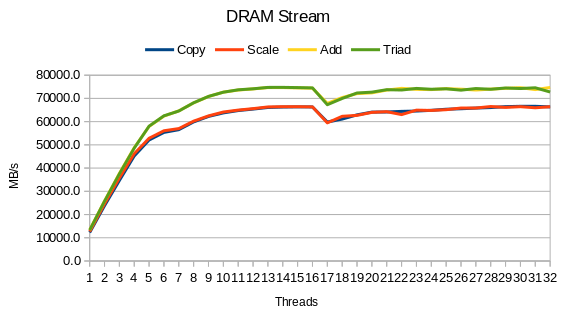
\includegraphics[scale=0.7]{DRAM_stream2.png}
\caption{DRAM Stream}
\end{figure}

\subsection{STREAM NVDIMM}
The stream NVDIMM benchmark measure the memory speed of the NVDIMM. This benchmark is the same as the STREAM DRAM benchmark mention above. The different is that the memory type have been changed from DRAM to NVDIMM.
The original code looks like this.
\begin{lstlisting}[caption=Description]
#ifndef STREAM_TYPE
#define STREAM_TYPE double
#endif

static STREAM_TYPE  a[STREAM_ARRAY_SIZE+OFFSET],
                    b[STREAM_ARRAY_SIZE+OFFSET],
                    c[STREAM_ARRAY_SIZE+OFFSET];
\end{lstlisting}
It have been changed into this. In addition the PMEMobjpool must be initiated in main method.
\begin{lstlisting}
PMEMobjpool *pop;
POBJ_LAYOUT_BEGIN(array);
POBJ_LAYOUT_TOID(array, double);
POBJ_LAYOUT_END(array);
TOID(double) a;
TOID(double) b;
TOID(double) c;

int main()
{
	const char path[] = "/mnt/pmem0-xfs/pool.obj";
	pop = pmemobj_create(path, LAYOUT_NAME, 10737418240, 0666);
	if (pop == NULL)
        	pop = pmemobj_open(path, LAYOUT_NAME);

        if (pop == NULL) {
                perror(path);
                exit(1);
        }
}

\end{lstlisting}

%\begin{figure}[!hbtp]
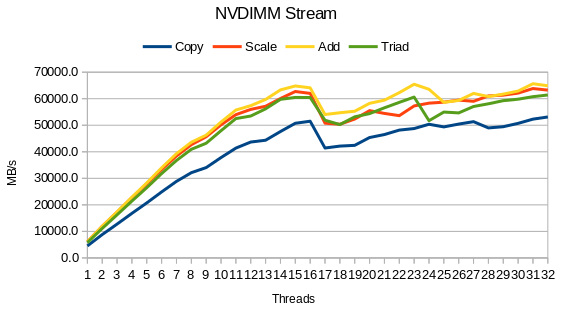
\includegraphics[scale=0.7]{NVDIMM_stream2.png}
%\caption{NVDIMM Stream}
%\end{figure}

\subsection{benchmark 3}
Graphs and tables below show the speed of a certain amount of NVDIMM threads while the rest of the threads are from DRAM to DRAM.
The test have been conducted by transfer data simultaneously from DRAM-DRAM and NVM-NVM.
All the threads are transferring the values of one array to another, all the arrays have 100 million elements of type double. This transfer happens 5000 times and the graphs shows the average of the first 200 iterations. This is done to ensure that all the threads can't finish early and make the remaining threads faster. The sum graphs shows the sum bandwidth of DRAM and NVM. Average graphs shows the average bandwidth of DRAM and NVM.

\subsubsection{The code}
The benchmark have three different program, the code is mostly the same except for the part where NVDIMM threads from NVDIMM-NVDIMM, DRAM-NVDIMM or NVDIMM-DRAM. 

The entire code is run in the main function except when it finds the current time, that is done in a different function.
The code begins with creating a memory pool and reads the parameters from command line. The parameters are how many threads are using the NVDIMM, the total amount of threads used and how many time the test will repeat itself. 
The code will then enter parallel area where one thread will create a 2d array where all the threads will save the time it took to copy the array. 

Every threads will then create their two arrays. The thread id will determine if both arrays will be DRAM array, or if one or two arrays will be NVDIMM array. Both arrays will be DRAM if the thread id is lower than the total amount of threads minus the number of NVDIMM threads. Thread ids equal or higher than that will either have one or both arrays stored in NVDIMM. All the arrays in all of the threads will be populated by random numbers. When a thread is done it will wait at a barrier until all the other threads are populating their threads.

\begin{lstlisting}[caption=Creation of DRAM and NVDIMM arrays]
if(thread_id < totalThreads-nvmThreads){
	//From DRAM to DRAM
	drm_read_array = (double*)malloc(ARRAY_LENGTH*sizeof(double));
	drm_write_array = (double*)malloc(ARRAY_LENGTH*sizeof(double));
	#pragma omp critical
	{
		for(i=0;i<ARRAY_LENGTH;i++){
			drm_read_array[i] = ((double)rand()/(double)(RAND_MAX));
			drm_write_array[i] = ((double)rand()/(double)(RAND_MAX));
		}
	}
}
else if(thread_id >= totalThreads-nvmThreads){
	//From NVDIMM to NVDIMM
	POBJ_ALLOC(pop, &nvm_read_array, double, sizeof(double) * ARRAY_LENGTH, NULL, NULL);
	POBJ_ALLOC(pop, &nvm_write_array, double, sizeof(double) * ARRAY_LENGTH, NULL, NULL);
	#pragma omp critical
	{
		for(i=0;i<ARRAY_LENGTH;i++){
			D_RW(nvm_read_array)[i] = ((double)rand()/(double)(RAND_MAX));
			D_RW(nvm_write_array)[i] = ((double)rand()/(double)(RAND_MAX));
		}
	}
}
\end{lstlisting}

Threads with DRAM arrays and threads with one or two NVDIMM array will split into their own part of the code with an if-sentence. All the threads will run the as many times as specified in the parameters and save the time each test takes in the 2d array that was created in the beginning. When they are done they will free up the memory and leave the parallel area. 

\begin{lstlisting}[caption=Threads running their test.]
if(thread_id < totalThreads-nvmThreads){
	//From DRAM to DRAM
	for(i=0;i<total_tests;i++){
		//Time start
		test_time[thread_id][i] = mysecond();
		for(j=0;j<ARRAY_LENGTH;j++){
			drm_write_array[j] = drm_read_array[j];
		}			
		//Time stop.
		test_time[thread_id][i] = mysecond() - test_time[thread_id][i];
	}
}
else if(thread_id >= totalThreads-nvmThreads){
	//From NVDIMM to NVDIMM
	for(i=0;i<total_tests;i++){
		//Time start
		test_time[thread_id][i] = mysecond2();
		for(j=0;j<ARRAY_LENGTH;j++)
			D_RW(nvm_write_array)[j] = D_RO(nvm_read_array)[j];		
		//Time stop.
		test_time[thread_id][i] = mysecond2() - test_time[thread_id][i];
	}
}
\end{lstlisting}

The code will then print the entire 2d array where the time measurements are stored to the terminal. Each line represent all the test done by one thread. In the beginning of each line the code will add either DRAM if both arrays are stored on DRAM. Or NVM if one or both arrays are stored on NVDIMM. When the program is done printing it will exit.

\subsubsection{NVM-NVM}
The tables below shows the result of the benchmark where one group of threads transfer from DRAM-DRAM and another group from NVDIMM-NVDIMM. The test result in the tables are the transfer speed in MB/s. The first table shows the combined transfer speed of all threads that are copying from DRAM-DRAM and the second table shows the combined speed of all the threads that are copying from NVDIMM-NVDIMM. 

The first line in the first table in figure 2 shows the combined transfer speed of the DRAM-DRAM copying where there are one thread copying from NVDIMM-NVDIMM. That means there are 15 threads that are copying from DRAM-DRAM. 
The first line in the second table shows the transfer speed of that one thread. The columns shows the the test numbers. The column with name the "1-20" shows the average transfer speed of the first 20 tests.
The third table in figure 3 shows the combined transfer speed of all the 16 threads in the first two tables. 
There is also a graph where all three tables are being represented.

One of the hopes by using NVDIMM and DRAM simultaneously was that there would be an increase in the transfer speed. But by comparing copy on figure 1 with the sum on figure 4 one can see that there has been no increase in transfer speed. Both graphs shows a transfer speed on around 65000 MB/s.

\begin{figure}[!hbtp]
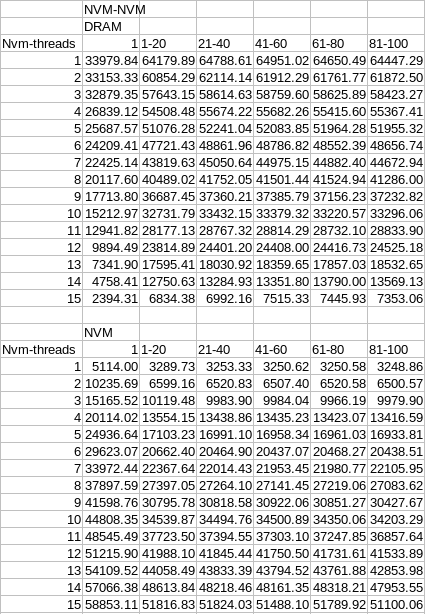
\includegraphics[scale=0.7]{NVM-NVM_table_p1_1-100_v3}
\caption{NVM-NVM 1-100 iteration, 16 threads total, 3rd version}
\end{figure}

\begin{figure}[!hbtp]
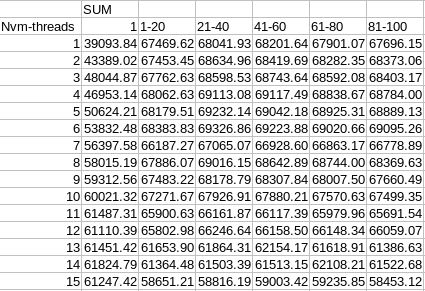
\includegraphics[scale=0.7]{NVM-NVM_table_p2_1-100_v3}
\caption{NVM-NVM 1-100 iteration, 16 threads total, 3rd version}
\end{figure}

\begin{figure}[!hbtp]
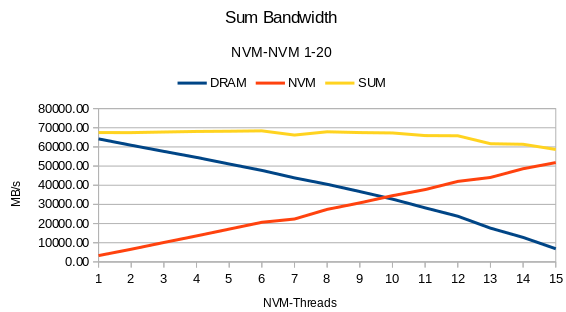
\includegraphics[scale=0.7]{NVM-NVM_Graph_1-20_v3}
\caption{NVM-NVM graph 1-20, 3rd version}
\end{figure}

\clearpage
\subsubsection{NVM-DRAM}
This benchmark is similar to the previous benchmark. The only difference is that some threads will transfer data from NVDIMM-DRAM instead of NVDIMM-NVDIMM.
\begin{figure}[!hbtp]
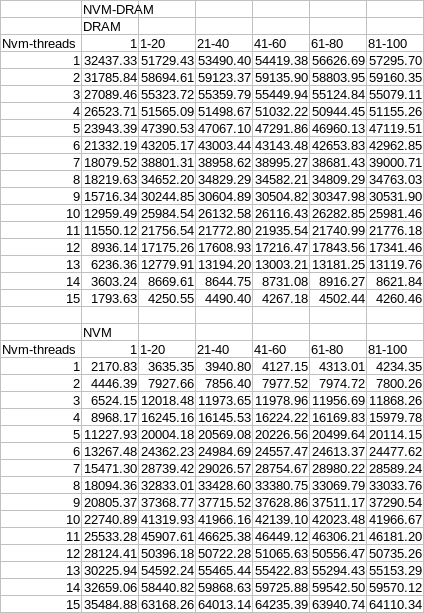
\includegraphics[scale=0.7]{NVM-DRAM_table_p1_1-100_v3}
\caption{NVM-DRAM 1-100 iteration, 3rd version}
\end{figure}

\begin{figure}[!hbtp]
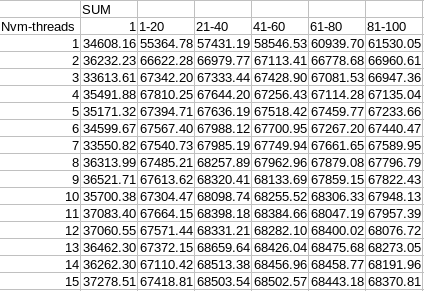
\includegraphics[scale=0.7]{NVM-DRAM_table_p2_1-100_v3}
\caption{NVM-DRAM 1-100 iteration, 3rd version}
\end{figure}

\begin{figure}[!hbtp]
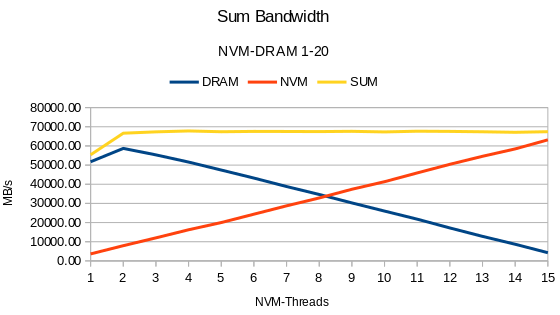
\includegraphics[scale=0.7]{NVM-DRAM_Graph_1-20_v3}
\caption{NVM-DRAM graph 1-20, 3rd version}
\end{figure}

\clearpage
\subsubsection{DRAM-NVM}
This benchmark is also similar to the other two benchmarks. This time some of the threads will transfer from DRAM-NVDIMM.
\begin{figure}[!hbtp]
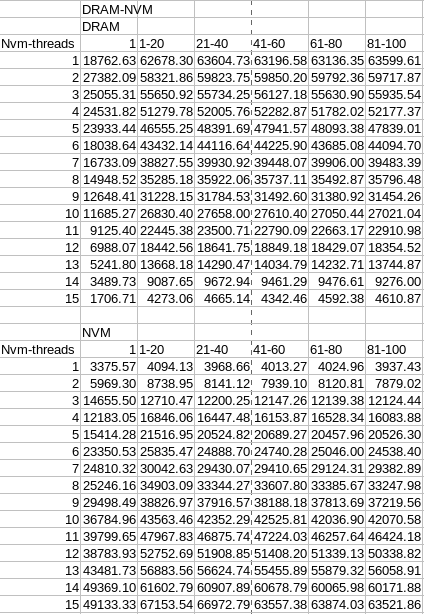
\includegraphics[scale=0.7]{DRAM-NVM_table_p1_1-100_v3}
\caption{DRAM-NVM 1-100 iteration, 3rd version}
\end{figure}

\begin{figure}[!hbtp]
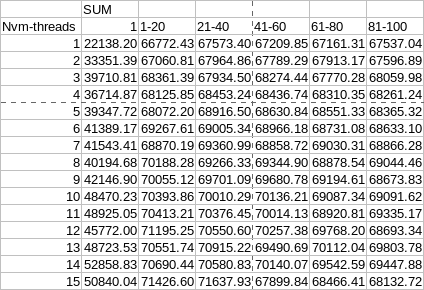
\includegraphics[scale=0.7]{DRAM-NVM_table_p2_1-100_v3}
\caption{DRAM-NVM 1-100 iteration, 3rd version}
\end{figure}

\begin{figure}[!hbtp]
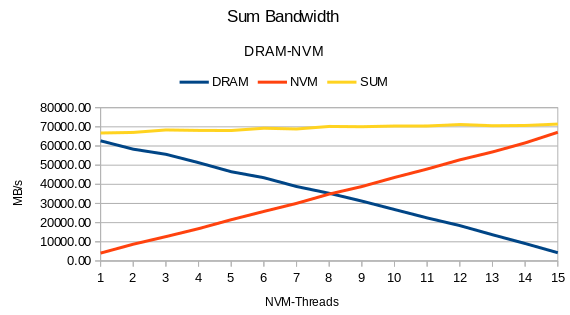
\includegraphics[scale=0.7]{DRAM-NVM_Graph_1-20_v3}
\caption{DRAM-NVM graph 1-20, 3rd version}
\end{figure}

%\clearpage
%\subsection{benchmark 4}
%stuff

\clearpage
\section{Simulation}
\subsection{DRAM only}
\begin{table}[!hbtp]
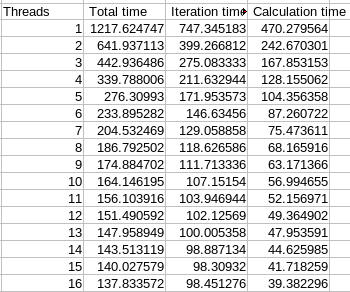
\includegraphics[scale=0.7]{DRAM_only_16M.png}
\caption{Simulation with only DRAM, n=16M}
\end{table}
The generation of data happens inside a while-loop that will repeat the generation and analyzing of data 5000 times. The total time is measured by taking the time before and after the while-loop. The analyzing time is measured the same way by taking the time before and after the analyzing part of the program. Data generation time is measured by subtracting the analyze time from the total time. All the time measurements are made inside a pragma omp singel so there are no reason to be worried if the mysecond-method is thead-safe. The mysecond-method have been copied from the original stream benchmark.
All the arrays used in the code have been subjected to first touch before the time is measured. 
\begin{lstlisting}[caption=while-loop]
#pragma omp single
{
	data_generation_time, = mysecond();
}
while( n<5000 ){
	#pragma omp barrier
	#pragma omp single
	{
		n++;
		diff=0.0;
		average = 0;
		//completes the first part of the formula.
		Wk_1_product = (omd + (d*Wk_1))*iN;
	}
	
	Data generation, see chapter 5.1.1
	
	#pragma omp barrier
	#pragma omp single
	{
		temp_x = xk_1;
		xk_1 = x;
		x = temp_x;
		//starting time measurement of calculation.
		temp_calc=mysecond();
	}
	
	Analyzing the data, see chapter 5.1.2
	
	#pragma omp barrier
	#pragma omp single
	{
		average *= iN;
		analyze_time+=mysecond()-temp_calc;
	}
}
#pragma omp single
{
	data_generation_time, = mysecond() - data_generation_time;
}
\end{lstlisting}
\begin{lstlisting}[caption=while-loop]
double mysecond(){
	struct timeval tp;
	struct timezone tzp;
	int i;
	i = gettimeofday(&tp,&tzp);
	return ( (double) tp.tv_sec + (double) tp.tv_usec * 1.e-6 );
}
\end{lstlisting}
%\clearpage
\subsubsection{Data generation}
The arrays x and xk\_1 are double arrays that have the length of 4'000'000 elements. CRS\_row\_ptr and CRS\_col\_idx are int arrray that have the length of 31'976'004 elements, CRS\_`values have the same length and a double array.
The code run through the x-array one time and xk\_1 twice. It also runs through CRS\_row\_ptr, CRS\_col\_idx and CRS\_values once. The formula for calculating memory traffic is 3*4'000'000+2*31'976'004 this would amount to 607 MB per iteration of the while-loop. 


\begin{lstlisting}[caption=Generation of data.]
#pragma omp for reduction(max:diff)
for( i=0; i<nodes; i++){
	x[i] = 0;
	for( j=CRS_row_ptr[i]; j<CRS_row_ptr[i+1]; j++)
		x[i] += CRS_values[j] * xk_1[CRS_col_idx[j]];
	x[i] *= d;
	x[i] += Wk_1_product;
	//Comuting the difference between x^k and x^k-1
	//and adds the biggest diff to diffX[thread_id]
	if( x[i]-xk_1[i] > diff ){
		diff = x[i] - xk_1[i];
	}
}
\end{lstlisting}

\begin{table}[!hbtp]
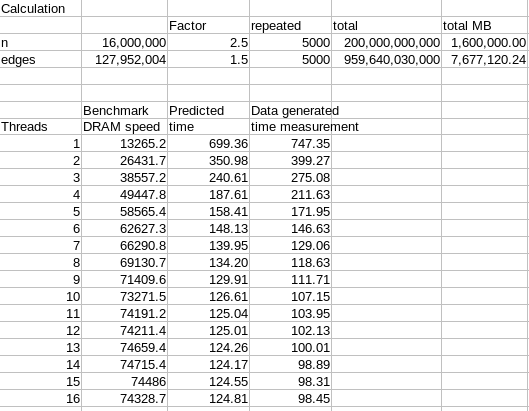
\includegraphics[scale=0.7]{DRAM_only_DataGeneration_16M.png}
\caption{Prediction of time taken for data generation, n=16M}
\end{table}

\clearpage
\subsubsection{Analyze}
The analyze part run through the nodes array five times and add all the elements to the average variable. The average variable is divided by the number of elements in array, this is shown in the code in chapter 5.1. The memory traffic will amount of 160MB per while-loop iteration.
\begin{lstlisting}[caption=Analyzing the data.]
//Analyse part
#pragma omp for reduction(+ : average)
	for(i=0;i<nodes;i++){
	average += xk_1[i];
}
#pragma omp for reduction(+ : average)
	for(i=0;i<nodes;i++){
	average += xk_1[i];
}
#pragma omp for reduction(+ : average)
	for(i=0;i<nodes;i++){
	average += xk_1[i];
}
#pragma omp for reduction(+ : average)
for(i=0;i<nodes;i++){
	average += xk_1[i];
}
#pragma omp for reduction(+ : average)
for(i=0;i<nodes;i++){
	average += xk_1[i];
}
\end{lstlisting}

\begin{table}[!hbtp]
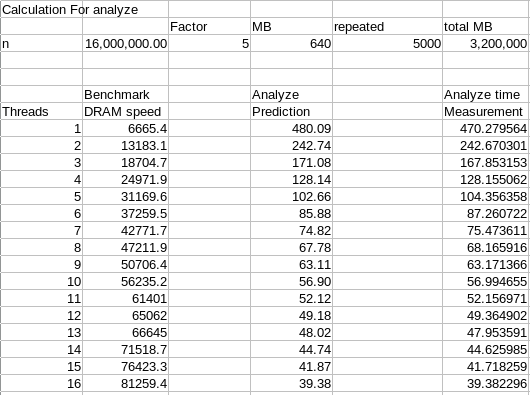
\includegraphics[scale=0.7]{DRAM_only_Analyze_16M.png}
\caption{Prediction of time taken for analyzing the data, n=16M}
\end{table}

\clearpage
\subsubsection{Stream benchmark, sum}
This benchmark is the STREAM benchmark with an added benchmark. The sum is found by adding all the elements into a single variable. The STREAM benchmark was changed by increasing several array from four to five and added the sum benchmark after the four other benchmark. 
The STREAM benchmark for NVDIMM is the same as the one described above, but the code has been changed so the benchmark will read and write to the NVDIMM.

\begin{table}[!hbtp]
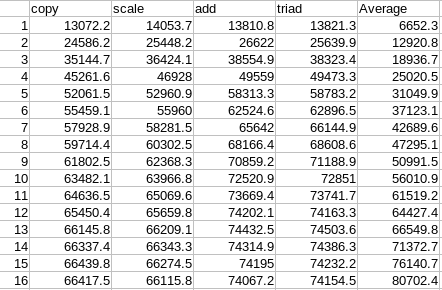
\includegraphics[scale=0.7]{Stream_benchmark.png}
\caption{New Stream benchmark, DRAM}
\end{table}

\begin{table}[!hbtp]
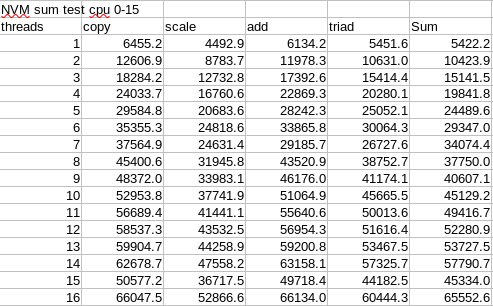
\includegraphics[scale=0.7]{Stream_NVM_sum.png}
\caption{New Stream benchmark, NVM}
\end{table}

\clearpage
\subsubsection{Calculation only} 
\begin{table}[!hbtp]
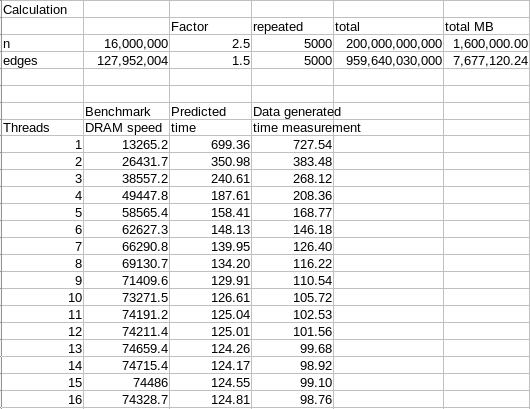
\includegraphics[scale=0.7]{Benchmark_only_prediction.png}
\caption{Prediction of time taken for calculation of the data, with a code that only do calculation}
\end{table}

\clearpage
\subsection{NVDIMM Analyze only}
\begin{table}[!hbtp]
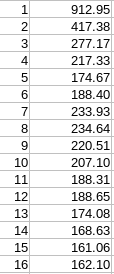
\includegraphics[scale=0.7]{NVDIMM_analyze_only}
\caption{Mearsurement of analyzations only on NVDIMM.}
\end{table}

\clearpage
\subsection{NVM simulation}
\subsubsection{Locks}
The program are divided into two parts, the calculation of data and the analyzing of the data that have been generated. The two parts synchronize by using two locks called lock\_a and lock\_b, lock\_a will start in unlocked state and lock\_b in locked state. When the two parts starts the analyzing part is put on hold by lock\_b until the calculation part has generated the first set of data. Then the calculation part will lock lock\_a, swap the pointers x and xk\_1 and then unlock lock\_b. The calculation part will then start the calculation of the next set of data, but wont swap pointers until analyzing part has transferred the content in xk\_1 to NVDIMM and unlocked lock\_a.

When the calculation part unlocks lock\_b the analyzing will start transferring data from xk\_1 to NVDIMM and unlock lock\_a when it's done with the transfer. The analyzing part will then start analyzing the data on NVDIMM. When its done it will encounter lock\_b and will wait there until calculation has a new set of data ready and has swapped the pointers.

Before and after the set lock in calculation and analyze part there is a time measurement that measure how long the threads have waited for the lock to be unlocked by the other part. All the individual times the threads have waited in calculation or analyze gets added to a variable called iteration\_idle\_time or transfer\_idle\_time that will be the total time the threads have waited. 

%lock_overview.png
\begin{figure}[!hbtp]
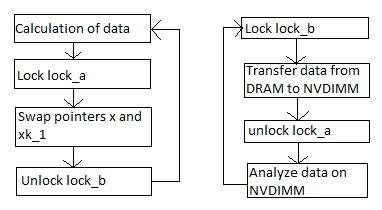
\includegraphics[scale=1]{lock_overview.png}
\caption{A simplified version of how lock works.}
\end{figure}

\begin{lstlisting}[caption=Calculation]
while( n<5000 ){ 
	#pragma omp barrier
	/*
		Calculation of Data
	*/
	#pragma omp single
	{
		temp_time = mysecond();
		omp_set_lock(&lock_a);
		iteration_idle_time += mysecond() - temp_time;

		temp_x = xk_1;
		xk_1 = x;
		x = temp_x;
		
		omp_unset_lock(&lock_b);
	}
}//end of while-loop
\end{lstlisting}
\begin{lstlisting}[caption=Analyze]
while(1==1){
	#pragma omp single
	{
		temp_time = mysecond();
		omp_set_lock(&lock_b);
		transfer_idle_time += mysecond() - temp_time;
		temp_time = mysecond();
		average=0.0;
	}
	/*
		Transfer of array from DRAM to NVDIMM
	*/
	#pragma omp single 
	{
		DRAM_to_NVM_time += mysecond() - temp_time;
		omp_unset_lock(&lock_a);
		temp_time = mysecond();
	}
	/*
		Analyzations of data
	*/
	}
	#pragma omp barrier
	#pragma omp single
	{
		Analyse_time += mysecond() - temp_time;
	}
	//if sentence for exiting while-loop.
	if(iteration_ongoing==0){
		break;
	}
}
\end{lstlisting}


\begin{table}[!hbtp]
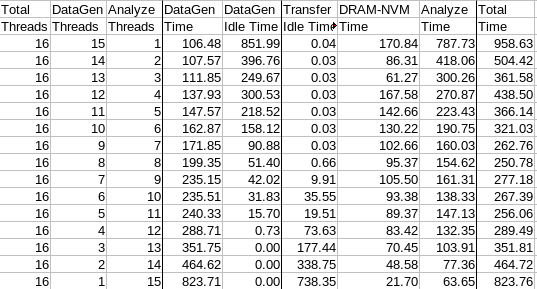
\includegraphics[scale=0.7]{Simulation_NVM_2.png}
\caption{Simulation with both NVDIMM and DRAM}
\end{table}

getconf LEVEL1\_DCACHE\_LINESIZE have been used to find the cacheline size in bytes.

\begin{table}[!hbtp]
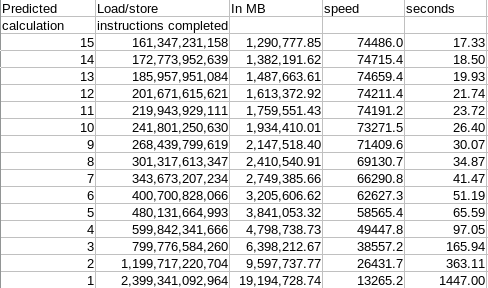
\includegraphics[scale=0.7]{Predicted_calculation.png}
\caption{Predicted calculationbased on papi.}
\end{table}

\begin{table}[!hbtp]
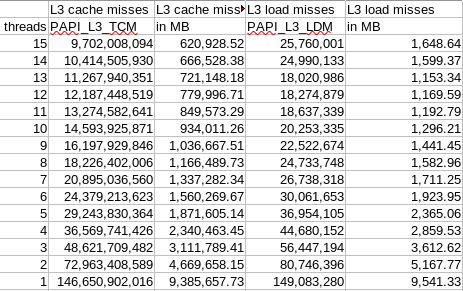
\includegraphics[scale=0.7]{Predicted_calculation_3.png}
\caption{Tried to split load and store misses. Server do not support store misses.}
\end{table}

\begin{table}[!hbtp]
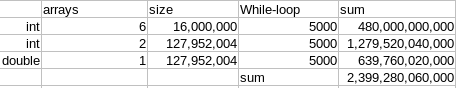
\includegraphics[scale=0.7]{Array-counting.png}
\caption{Manually counted the number of int and double tranfers.}
\end{table}

\begin{table}[!hbtp]
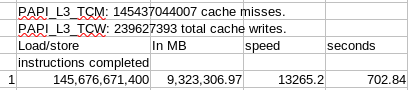
\includegraphics[scale=0.7]{Predicted_calculation_2.png}
\caption{Predicted calculationbased on papi with L3.}
\end{table}

\begin{table}[!hbtp]
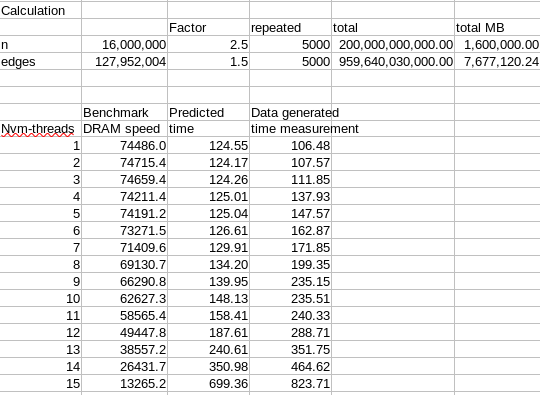
\includegraphics[scale=0.7]{Datagen_prediction_NVM.png}
\caption{Time prediction, data generation}
\end{table}

\begin{table}[!hbtp]
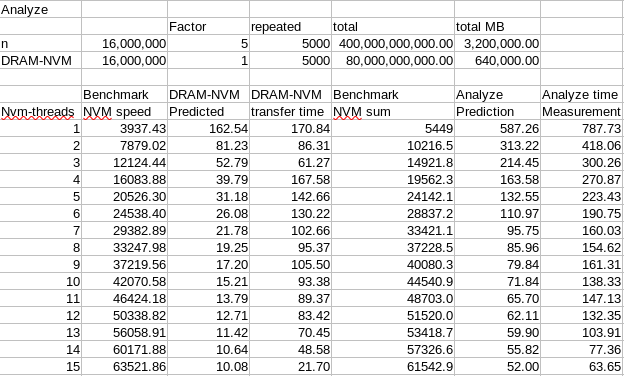
\includegraphics[scale=0.7]{Analyze_prediction_NVM.png}
\caption{Time prediction, transfer and analyze}
\end{table}

\clearpage
\subsection{2D-array test}
\begin{lstlisting}[caption=Kildekode]
https://github.com/SveinGunnar/Master_Thesis_2020/tree/master/ArrayCopyTest
\end{lstlisting}
\begin{table}[!hbtp]
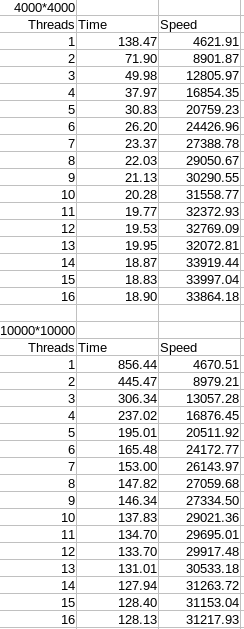
\includegraphics[scale=0.7]{2D_array_test.png}
\caption{2D-Array test}
\end{table}

\clearpage
\section{Large array benchmark}
The size of data that must be analyzed keeps increasing year after year and the prize for DRAM are not getting cheaper. NVDIMM offer a lot of storage at a cheaper prize. This opens the opportunity to save money by offloading some of the data to the NVDIMM where the data will be analyzed the same way as the data on the DRAM. The downside to this strategy is that NVDIMM is slower than DRAM so the question is how much data can be offloaded to NVDIMM. If the user offload too much data to NVDIMM then the threads working on analyzing the data on DRAM will be idle while waiting for NVDIMM threads to complete.
\\
\\
Calculation\\
This program have an two dimensional array filled with data. The program start at element (1,1) of the array where it sum ups all of its eight neighbors and then takes the average. The result is stored in the same position in another two dimensional array. The program does this for every element between (1,1) and (m-2,n-2).
\clearpage
Formula
\[
    \frac{dram\_data-nvdimm\_data}{dram\_speed} = \frac{nvdimm\_data}{nvdimm\_speed}    
\]
\[
    nvdimm\_data = \frac{nvdimm\_speed*dram\_data}{nvdimm\_speed+dram\_speed}
\]
\\
\\
\begin{table}[!hbtp]
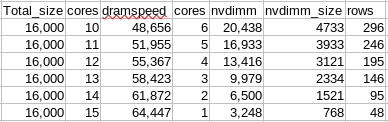
\includegraphics[scale=0.7]{Formula_calculation.png}
\caption{Formula calculation}
\end{table}

\begin{table}[!hbtp]
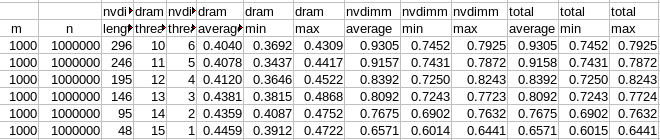
\includegraphics[scale=0.7]{Formula_First_version.png}
\caption{First version}
\end{table}

\begin{table}[!hbtp]
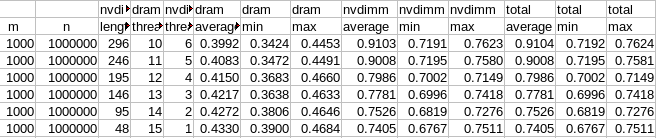
\includegraphics[scale=0.7]{Formula_Second_version.png}
\caption{Second version}
\end{table}

\subsection{First version}
There are two groups of threads that works in parallel in this program. The first group of threads works on the part of the data that is stored on DRAM and the other works on the data strored on NVDIMM. One thread in each group works on data that borders with the other group. In the DRAM group that will be the last thread and in the NVDIMM group that would be the first group. 
\begin{lstlisting}[caption=First version]
while(k<K_length){
	#pragma omp barrier
	#pragma omp single
	{
		total_time[k] = mysecond();
	}
	#pragma omp barrier
	if( thread_id < dram_threads ){
		//for the thread bordering on nvdimm thread.
		if( thread_id==(dram_threads-1) ){
			individual_time[thread_id] = mysecond();
			for( i=slice_start; i<slice_end-1; i++){
				for( j=1; j<nMinusOne; j++){
					temp = A[i-1][j-1] + A[i-1][j] + A[i-1][j+1]+
							 A[i][j-1]        +        A[i][j+1]+
						   A[i+1][j-1] + A[i+1][j] + A[i+1][j+1];
					B[i][j] = temp*inverseEigth;
				}
			}

			i = slice_end-1;
			for( j=1; j<nMinusOne; j++){
				temp = A[i-1][j-1] + A[i-1][j] + A[i-1][j+1]+
						 A[i][j-1]        +        A[i][j+1]+
					D_RO(C)[i*n+j] + D_RO(C)[i*n+j] + D_RO(C)[i*n+j];
				B[i][j] = temp*inverseEigth;
			}
			individual_time[thread_id] = mysecond() - individual_time[thread_id];
		}else{
			//For all the threads not bordering with nvdimm.
			individual_time[thread_id] = mysecond();
			for( i=slice_start; i<slice_end; i++){
				for( j=1; j<nMinusOne; j++){
					temp = A[i-1][j-1] + A[i-1][j] + A[i-1][j+1]+
							 A[i][j-1]        +        A[i][j+1]+
						   A[i+1][j-1] + A[i+1][j] + A[i+1][j+1];
					B[i][j] = temp*inverseEigth;
				}
			}
			individual_time[thread_id] = mysecond() - individual_time[thread_id];
		}
	}else{
		if( thread_id==dram_threads ){
			individual_time[thread_id] = mysecond();
			i=0;
			for( j=1; j<nMinusOne; j++){
			temp = A[dram_part-1][j-1]+A[dram_part-1][j]+A[dram_part-1][j+1]+
				   D_RO(C)[i*n+(j-1)]            +            D_RO(C)[i*n+(j+1)]+
				   D_RO(C)[(i+1)*n+(j-1)] + D_RO(C)[(i+1)*n+j] + D_RO(C)[(i+1)*n+(j+1)];
			D_RW(D)[i*n+j] = temp*inverseEigth;
		}
			for( i=slice_start+1; i<slice_end-1; i++){
				for( j=1; j<nMinusOne; j++){
					temp =  D_RO(C)[(i-1)*n+(j-1)] + D_RO(C)[(i-1)*n+j] + D_RO(C)[(i-1)*n+(j+1)]+
							D_RO(C)[i*n+(j-1)]            +					  D_RO(C)[i*n+(j+1)]+
							D_RO(C)[(i+1)*n+(j+1)] + D_RO(C)[(i+1)*n+j] + D_RO(C)[(i+1)*n+(j+1)];
					D_RW(D)[i*n+j] = temp*inverseEigth;
				}
			}
			individual_time[thread_id] = mysecond() - individual_time[thread_id];
		}else{
			individual_time[thread_id] = mysecond();
			for( i=slice_start; i<slice_end; i++){
				for( j=1; j<nMinusOne; j++){
					temp =  D_RO(C)[(i-1)*n+(j-1)] + D_RO(C)[(i-1)*n+j] + D_RO(C)[(i-1)*n+(j+1)]+
							D_RO(C)[i*n+(j-1)]            +            		  D_RO(C)[i*n+(j+1)]+
							D_RO(C)[(i+1)*n+(j-1)] + D_RO(C)[(i+1)*n+j] + D_RO(C)[(i+1)*n+(j+1)];
					D_RW(D)[i*n+j] = temp*inverseEigth;
				}
			}
			individual_time[thread_id] = mysecond() - individual_time[thread_id];
		}
	}
	#pragma omp barrier
	#pragma omp single
	{
		total_time[k] = mysecond() - total_time[k];
		dram_time[k]=individual_time[0];
		for(i=1;i<dram_threads;i++){
			if(dram_time[k]<individual_time[i])
				dram_time[k]=individual_time[i];
		}
		nvdimm_time[k]=individual_time[dram_threads];
		for(i=dram_threads+1;i<dram_threads+nvdimm_threads;i++){
			if(nvdimm_time[k]<individual_time[i])
				nvdimm_time[k]=individual_time[i];
		}
		k++;
	}
	#pragma omp barrier
}//End of while
\end{lstlisting}

\subsection{Second version}
\begin{lstlisting}[caption=Second version]
while(k<K_length){
	#pragma omp barrier
	#pragma omp single
	{
		total_time[k] = mysecond();
	}
	#pragma omp barrier
	if( thread_id < dram_threads ){
		individual_time[thread_id] = mysecond();
		for( i=slice_start; i<slice_end; i++){
			for( j=1; j<nMinusOne; j++){
				temp = A[i-1][j-1] + A[i-1][j] + A[i-1][j+1]+
						A[i][j-1]       +       A[i][j+1]+
						A[i+1][j-1] + A[i+1][j] + A[i+1][j+1];
				B[i][j] = temp*inverseEigth;
			}
		}
		individual_time[thread_id] = mysecond() - individual_time[thread_id];
	}else{
		individual_time[thread_id] = mysecond();
		for( i=slice_start; i<slice_end; i++){
			for( j=1; j<nMinusOne; j++){
				temp = D_RO(C)[(i-1)*n+(j-1)] + D_RO(C)[(i-1)*n+j] + D_RO(C)[(i-1)*n+(j+1)]+
						D_RO(C)[i*n+(j-1)]            +            D_RO(C)[i*n+(j+1)]+
						D_RO(C)[(i+1)*n+(j-1)] + D_RO(C)[(i+1)*n+j] + D_RO(C)[(i+1)*n+(j+1)];
				D_RW(D)[i*n+j] = temp*inverseEigth;
			}
		}
		individual_time[thread_id] = mysecond() - individual_time[thread_id];
	}
	#pragma omp barrier
	#pragma omp single
	{
		total_time[k] = mysecond() - total_time[k];
		dram_time[k]=individual_time[0];
		for(i=1;i<dram_threads;i++){
			if(dram_time[k]<individual_time[i])
				dram_time[k]=individual_time[i];
		}
		nvdimm_time[k]=individual_time[dram_threads];
		for(i=dram_threads+1;i<dram_threads+nvdimm_threads;i++){
			if(nvdimm_time[k]<individual_time[i])
				nvdimm_time[k]=individual_time[i];
		}
		k++;
	}
	#pragma omp barrier
}//End of while
\end{lstlisting}

\begin{table}[!hbtp]
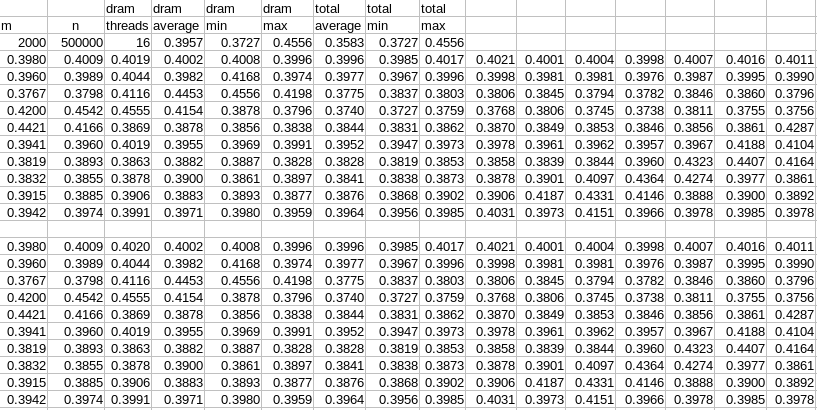
\includegraphics[scale=0.6]{First_version_DRAM_only_17_9_21.png}
\caption{First version, dram only}
\end{table}

\begin{table}[!hbtp]
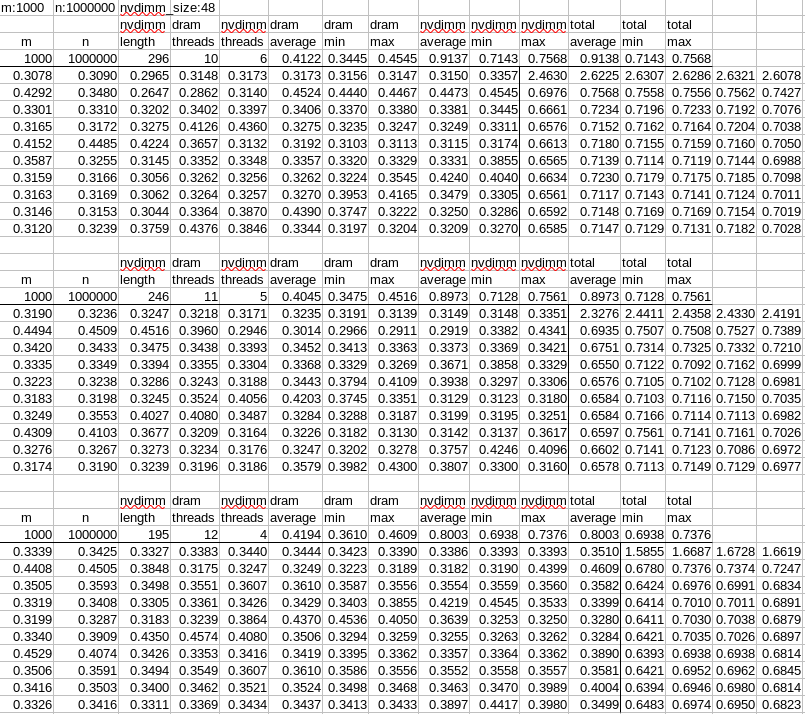
\includegraphics[scale=0.6]{first_version_more_detailed_1.png}
\caption{First version, more detailed 1}
\end{table}

\begin{table}[!hbtp]
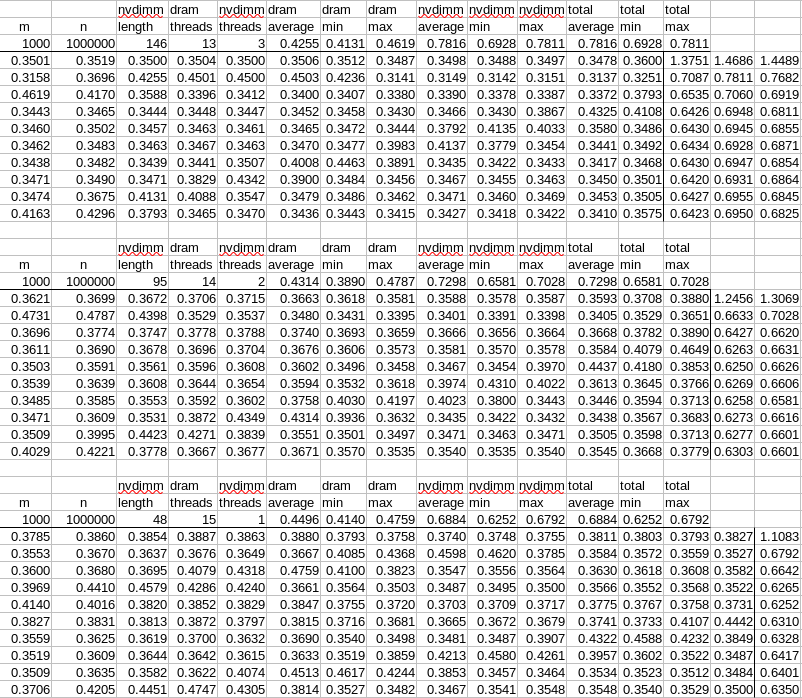
\includegraphics[scale=0.6]{first_version_more_detailed_2.png}
\caption{First version, more detailed 2.}
\end{table}

\begin{table}[!hbtp]
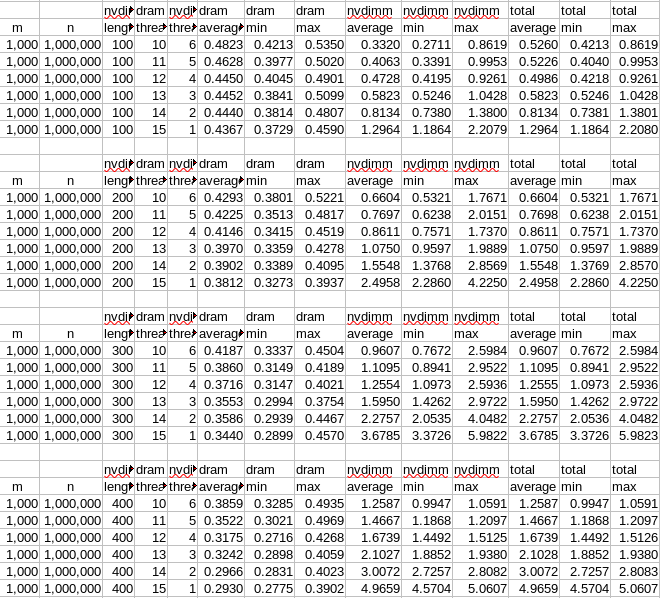
\includegraphics[scale=0.7]{Large_array_test_first_version_v5.png}
\caption{First version.}
\end{table}

\begin{table}[!hbtp]
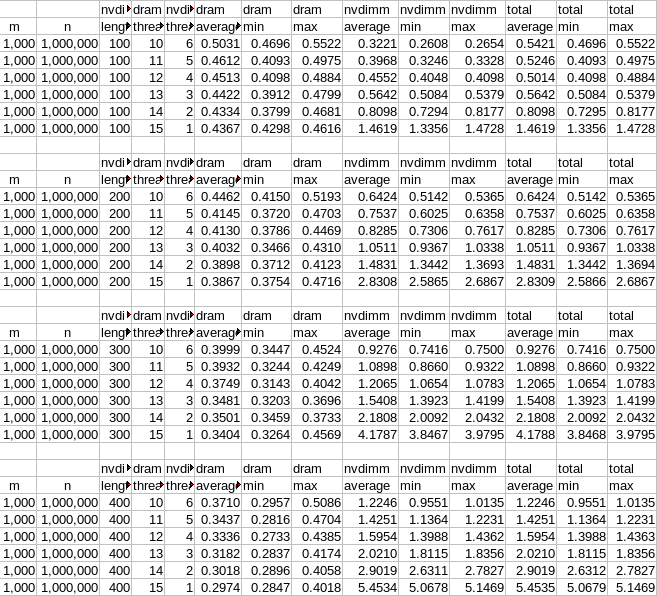
\includegraphics[scale=0.7]{Large_array_test_second_version_v3.png}
\caption{Second version.}
\end{table}

\begin{table}[!hbtp]
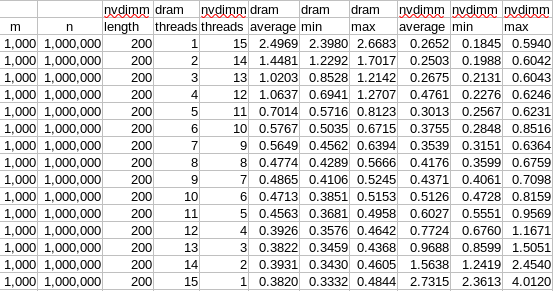
\includegraphics[scale=0.7]{Large_array_test_first_version_v2.png}
\caption{First version. OLD}
\end{table}

\begin{table}[!hbtp]
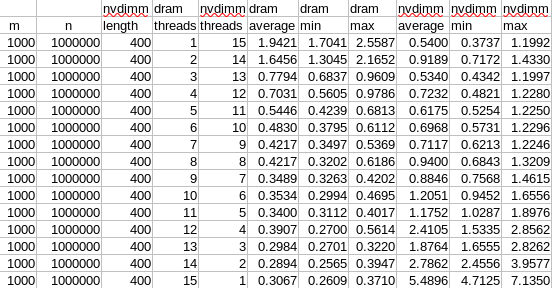
\includegraphics[scale=0.7]{Large_array_test_first_version_v3.png}
\caption{First version. OLD}
\end{table}

\begin{table}[!hbtp]
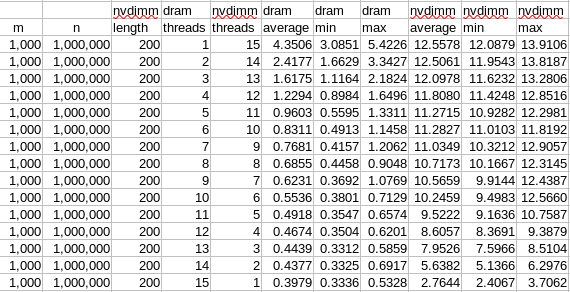
\includegraphics[scale=0.7]{Large_array_test_second_version_v2.png}
\caption{Second version. OLD}
\end{table}

\begin{table}[!hbtp]
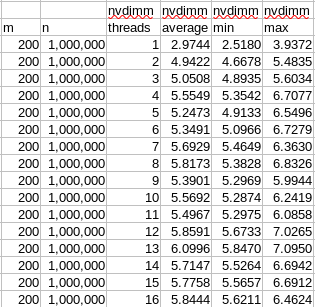
\includegraphics[scale=0.7]{Large_array_test_second_version_NVDIMM_only_v2.png}
\caption{NVDIMM only of second version. OLD}
\end{table}

\begin{table}[!hbtp]
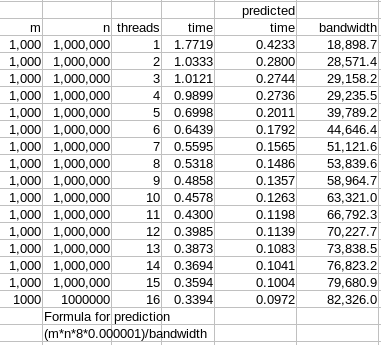
\includegraphics[scale=0.7]{DRAM_only_on_n50.png}
\caption{DRAM only on n50. OLD}
\end{table}

\
\
\
\
\clearpage
\printbibliography

% PageRank_iterations

%latex -interaction=nonstopmode %.tex|bibtex %.aux|latex -interaction=nonstopmode %.tex|latex -interaction=nonstopmode %.tex|xdvi %.dvi
\end{document}               % End of document.